\documentclass[conference]{IEEEtran}
\IEEEoverridecommandlockouts

\usepackage{cite}
\usepackage{amsmath,amssymb,amsfonts}
\usepackage{graphicx}
\usepackage{textcomp}
\usepackage{xcolor}
\usepackage{booktabs}
\usepackage{multirow}
\usepackage{xurl}
\usepackage{listings}
\usepackage{tikz}
\graphicspath{{test/results/}}
\usetikzlibrary{shapes.geometric,arrows.meta,positioning,fit,backgrounds}

\lstset{basicstyle=\ttfamily\footnotesize, breaklines=true,
        frame=single, columns=fullflexible}

\def\BibTeX{{\rm B\kern-.05em{\sc i\kern-.025em b}\kern-.08em
    T\kern-.1667em\lower.7ex\hbox{E}\kern-.125emX}}

\begin{document}

\title{TinyML Visual Alarm System:\\
On-Device Person Detection with Notification}

\author{%
\IEEEauthorblockN{Andrea Renelli}
\IEEEauthorblockA{%
  \textit{Laboratory of Internet of Things, University of Trento}\\
  andrea.renelli@studenti.unitn.it}
}

\maketitle

\begin{abstract}
Deploying ML inference directly on microcontrollers eliminates bandwidth overhead and privacy exposure inherent in cloud-based video surveillance. The main challenge is fitting a viable vision model within the severe memory and compute constraints of embedded hardware while maintaining alarm-grade precision. This paper presents a Smart Visual Alarm System on the ESP32-S3-EYE that addresses this challenge through fully on-device person detection: a quantized MobileNetV1 running under TensorFlow Lite for Microcontrollers achieves 88.9\% precision at a false-alarm rate of only 7.3\%, with end-to-end inference latency of 351 ms ($\approx$2.85 FPS) on the embedded hardware. A three-frame moving-average filter further suppresses spurious triggers in live video. Alarm events are published via MQTT to a Python backend that delivers real-time Telegram notifications. Evaluated on 123,287 COCO 2017 images, the system achieves ROC-AUC = 0.814 and AP = 0.852.
\end{abstract}

\begin{IEEEkeywords}
ESP32-S3-EYE, TFLite Micro, person detection, MQTT, Telegram Bot, IoT,
edge AI, TinyML
\end{IEEEkeywords}

% ─────────────────────────────────────────────────────────────────────────────
\section{Introduction}
\label{sec:intro}

The proliferation of low-cost cameras in homes, offices, and public spaces has made video-based surveillance a cornerstone of modern security systems. Traditionally, these systems rely on continuous video streaming to remote servers or cloud platforms, where inference is performed centrally. This architecture, however, carries two fundamental costs. First, transmitting raw video over a network exposes sensitive visual data to interception, storage by third parties, and potential misuse, a serious privacy concern in residential and workplace deployments where occupants have a reasonable expectation not to be recorded and analysed off-premises, as exemplified by the well-documented Amazon Ring case~\cite{ftc2023ring}. Second, continuous video streaming is bandwidth-intensive: a single 720p camera at modest quality can consume several Mbps of uplink, making cloud-based inference economically and practically unviable in bandwidth-constrained or large-scale deployments. Edge computing addresses both issues by pushing inference directly to the data source, so that only high-level semantic events, rather than raw pixels, ever leave the device.

Realising vision-based inference on embedded hardware is, however, far from straightforward. Microcontrollers (MCUs) typically operate with tens to hundreds of kilobytes of SRAM, no dedicated GPU, and clock speeds in the hundreds of MHz, orders of magnitude below the resources assumed by standard deep learning frameworks. Fitting a convolutional neural network capable of meaningful person detection within these constraints requires aggressive model compression (quantisation, architecture search) and careful memory management, all while meeting real-time latency requirements suitable for an alarm application.
A complete Smart Visual Alarm System is presented that addresses the above challenges end-to-end on a single embedded device. The main contributions are: (i) a fully on-device person detection pipeline on the ESP32-S3-EYE, combining a quantized MobileNetV1 with a three-frame moving-average filter for robust alarm triggering without any cloud dependency, (ii) a lightweight MQTT-based event notification architecture in which raw video never leaves the device and only compact JSON descriptors are transmitted, (iii) a systematic evaluation on 123,287 COCO 2017 images demonstrating ROC-AUC $= 0.814$, AP $= 0.852$, and $88.9\%$ precision at a false-alarm rate of $7.3\%$, with a hardware inference latency of $351$ ms on the target MCU.
% ─────────────────────────────────────────────────────────────────────────────
\section{System Architecture}
\label{sec:arch}

In this section the architecture of the system is detailed, starting from
the high-level overview of the three tiers, followed by a description of
the target hardware platform, the on-device inference pipeline, the
detection and alarm logic, and finally the backend notification mechanism.

\subsection{Overview}

The system comprises three tiers (Fig.~\ref{fig:arch}): the
ESP32-S3-EYE firmware, a Mosquitto MQTT broker, and a Python/Telegram
backend. A central design principle is that raw video frames never leave
the device: only compact JSON event descriptors are transmitted over the
network. This on-device processing ensures that no visual data is
exposed to interception or third-party storage, directly addressing the
privacy concerns described in Section~\ref{sec:intro}. The firmware
connects to the broker over Wi-Fi using MQTT QoS~1, which guarantees
at-least-once delivery of every alarm event even in the presence of
transient network failures. The notification pipeline follows a
\emph{Publisher-Subscriber} pattern: the firmware publishes alarm events
to a named MQTT topic, while the Python backend subscribes
asynchronously, decoupling event generation from notification consumers
and allowing additional subscribers (dashboards, logging services) to be
attached without modifying the firmware.

\begin{figure}[h]
\centering
\resizebox{\columnwidth}{!}{%
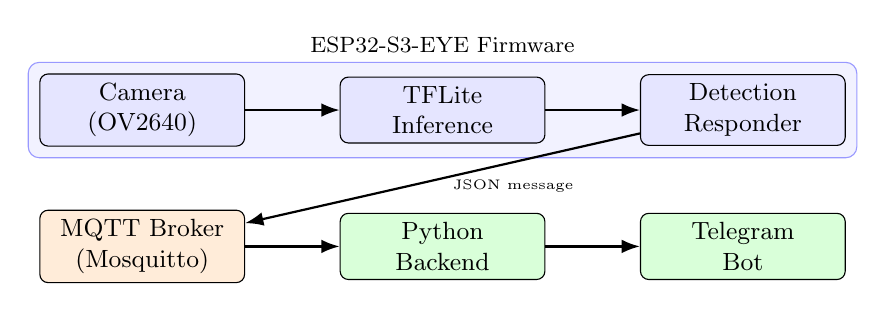
\begin{tikzpicture}[
  box/.style={draw, rounded corners=3pt, minimum width=2.6cm,
              minimum height=0.7cm, align=center, font=\small},
  arr/.style={-Latex, thick},
  node distance=0.5cm and 1.2cm
]
  \node[box, fill=blue!10] (cam)  {Camera\\(OV2640)};
  \node[box, fill=blue!10, right=of cam] (inf)  {TFLite\\Inference};
  \node[box, fill=blue!10, right=of inf] (resp) {Detection\\Responder};
  \node[box, fill=orange!15, below=0.8cm of cam] (mqtt) {MQTT Broker\\(Mosquitto)};
  \node[box, fill=green!15, right=of mqtt] (py) {Python\\Backend};
  \node[box, fill=green!15, right=of py]   (tg) {Telegram\\Bot};
  \draw[arr] (cam) -- (inf);
  \draw[arr] (inf) -- (resp);
  \draw[arr] (resp) -- node[right,yshift=-3pt,font=\tiny]{JSON message} (mqtt);
  \draw[arr] (mqtt) -- (py);
  \draw[arr] (py) -- (tg);
  \begin{pgfonlayer}{background}
    \node[draw=blue!40, fill=blue!5, rounded corners,
          fit=(cam)(inf)(resp), inner sep=4pt,
          label={[font=\footnotesize]above:ESP32-S3-EYE Firmware}] {};
  \end{pgfonlayer}
\end{tikzpicture}
}
\caption{System architecture. Raw video stays on-device: only JSON alarm
         events are published over MQTT.}
\label{fig:arch}
\end{figure}

\subsection{Hardware Platform: ESP32-S3-EYE}

The target hardware is the ESP32-S3-EYE development board by Espressif
Systems \cite{esp32s3eye}, shown in Fig.~\ref{fig:esp32}. The board
integrates all the components required for a self-contained vision-based
edge inference system on a single compact module. The main
specifications are summarised in Table~\ref{tab:hw}.

\begin{table}[h]
\centering
\caption{ESP32-S3-EYE hardware specifications.}
\label{tab:hw}
\begin{tabular}{ll}
\hline
\textbf{Component} & \textbf{Specification} \\
\hline
SoC            & ESP32-S3, dual-core Xtensa LX7 @ 240\,MHz \\
On-chip SRAM   & 512\,KB \\
External PSRAM & 8\,MB (OPI PSRAM) \\
Flash          & 8\,MB \\
Camera         & OV2640, up to 2\,MP \\
Connectivity   & Wi-Fi 802.11 b/g/n, Bluetooth 5.0 \\
Display        & 1.3-inch LCD (240$\times$240) \\
Microphone     & Digital PDM microphone \\
Power supply   & USB Type-C, 5\,V \\
\hline
\end{tabular}
\end{table}

The dual-core LX7 processor, combined with 8\,MB of PSRAM, makes the
ESP32-S3-EYE particularly well suited for TinyML inference: one core
can be dedicated to camera capture and Wi-Fi communication, while the
other runs the inference loop, and the large PSRAM accommodates the
tensor arena and intermediate feature maps that would otherwise exhaust
the on-chip SRAM.

\begin{figure}[h]
  \centering
  \includegraphics[width=\columnwidth]{esp32s3eye.jpg}
  \caption{The ESP32-S3-EYE development board used in this work.}
  \label{fig:esp32}
\end{figure}

\subsection{On-Device Inference}

TFLite Micro \cite{tflitemicro} operates on a statically allocated
100\,KB tensor arena placed in PSRAM to preserve on-chip SRAM for the
RTOS and network stacks. Input images are resized to $96\!\times\!96$
pixels and converted to signed 8-bit integers before feeding the
quantized MobileNetV1 model. The model outputs a \emph{person score}
dequantised to float.

\subsubsection{MobileNetV1 Architecture}

MobileNetV1 \cite{mobilenet} is a lightweight convolutional neural
network designed for deployment on resource-constrained devices. Rather
than relying on standard convolutions throughout, it introduces
\emph{depthwise separable convolutions} as the main building block. A
depthwise separable convolution factorises a standard $k{\times}k$
convolution into two sequential operations: a per-channel $3{\times}3$
\emph{depthwise} filter, which applies a single filter to each input
channel independently, followed by a $1{\times}1$ \emph{pointwise}
convolution that linearly combines the outputs across channels. This
factorisation yields a reduction in multiply-accumulate operations
(MACs) with respect to a standard convolution of:
\begin{equation}
  \frac{\text{DW-Sep MACs}}{\text{Std Conv MACs}}
  = \frac{1}{C_o} + \frac{1}{k^2}
  \approx \frac{1}{9} \quad (k{=}3,\; C_o \gg 1)
  \label{eq:dwsep}
\end{equation}
making MCU deployment feasible without a substantial loss in
representational capacity.

The full architecture, illustrated in Fig.~\ref{fig:mobilenet}, is
structured as follows. The network opens with a single standard
$3{\times}3$ convolution with stride 2, the only layer of its kind in
the entire model. This is followed by 13 repeated depthwise separable
blocks, each consisting of a $3{\times}3$ depthwise convolution and a
$1{\times}1$ pointwise convolution, with batch normalisation and ReLU6
activation applied after each convolution. ReLU6, defined as
$\min(\max(0,x),6)$, is preferred over plain ReLU because its bounded
output improves numerical stability under fixed-point quantisation.
Spatial downsampling is achieved through strided depthwise convolutions
rather than max pooling, preserving more spatial information. The
network closes with a global average pooling layer that collapses the
spatial dimensions, followed by a fully connected layer (or equivalently
a $1{\times}1$ convolution) for classification. A \emph{depth
multiplier} hyperparameter $\alpha \in (0,1]$ uniformly scales the
number of channels in each layer, allowing a continuous trade-off
between accuracy and computational cost. The deployed model uses
$\alpha\!=\!0.25$, yielding 213,272 parameters and ${\approx}7.2$\,MMAC.

\begin{figure}[h]
\centering
\resizebox{\columnwidth}{!}{%
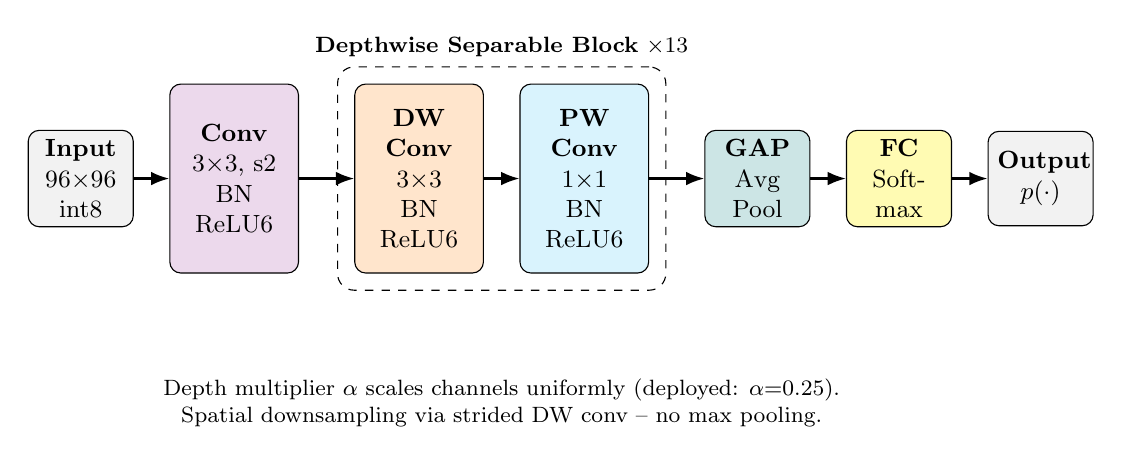
\begin{tikzpicture}[
  font=\small,
  node distance=0.35cm and 0.45cm,
  box/.style={draw, rounded corners=4pt, minimum width=1.5cm,
              minimum height=2.4cm, align=center, text width=1.4cm},
  boxsm/.style={draw, rounded corners=4pt, minimum width=1.1cm,
                minimum height=1.6cm, align=center, text width=1.0cm,
                font=\scriptsize},
  boxbn/.style={draw, rounded corners=4pt, minimum width=0.7cm,
                minimum height=1.6cm, align=center, text width=0.65cm,
                font=\scriptsize},
  io/.style={draw, rounded corners=4pt, minimum width=1.2cm,
             minimum height=1.2cm, align=center, text width=1.1cm},
  arr/.style={-Latex, thick},
  dashrect/.style={draw, dashed, rounded corners=6pt, inner sep=6pt}
]

\node[io, fill=gray!10] (input)
  {\textbf{Input}\\96$\times$96\\int8};

\node[box, fill=violet!15, right=of input] (conv1)
  {\textbf{Conv}\\3$\times$3, s2\\BN\\ReLU6};

\draw[arr] (input) -- (conv1);

\node[box, fill=orange!20, right=0.7cm of conv1] (dw)
  {\textbf{DW Conv}\\3$\times$3\\BN\\ReLU6};
\node[box, fill=cyan!15, right=of dw] (pw)
  {\textbf{PW Conv}\\1$\times$1\\BN\\ReLU6};

\draw[arr] (conv1) -- (dw);
\draw[arr] (dw)    -- (pw);

\node[dashrect, fit=(dw)(pw),
      label={[font=\footnotesize]above:\textbf{Depthwise Separable Block} $\times 13$}]
      (dsbox) {};

\node[io, fill=teal!20, right=0.7cm of pw] (gap)
  {\textbf{GAP}\\Avg\\Pool};
\draw[arr] (pw) -- (gap);

\node[io, fill=yellow!30, right=of gap] (fc)
  {\textbf{FC}\\Soft-\\max};
\draw[arr] (gap) -- (fc);

\node[io, fill=gray!10, right=of fc] (output)
  {\textbf{Output}\\$p(\cdot)$};
\draw[arr] (fc) -- (output);

\node[below=1.0cm of dsbox, font=\footnotesize, align=center] (note)
  {Depth multiplier $\alpha$ scales channels uniformly (deployed: $\alpha{=}0.25$).\\
   Spatial downsampling via strided DW conv -- no max pooling.};

\end{tikzpicture}
}
\caption{MobileNetV1 architecture. One standard convolution opens the
         network. Thirteen depthwise separable blocks follow, each consisting
         of a $3{\times}3$ depthwise conv, a $1{\times}1$ pointwise
         conv, batch normalisation, and ReLU6 activation. Global average
         pooling and a fully connected softmax classifier close the
         network.}
\label{fig:mobilenet}
\end{figure}



The shipped model uses \emph{post-training linear quantization}
\cite{tflitemicro}: each weight is mapped to a signed 8-bit integer via
$r = S(q-Z)$, where $S$ is a per-channel scale and $Z$ is the
zero-point. This compresses storage from ${\approx}1{,}174$\,KB
(float32 equivalent) to 293.5\,KB on flash, a $4{\times}$ reduction,
without additional training.

\subsection{Detection Logic and Alarm Trigger}

A moving-average filter with window $W\!=\!3$ frames smooths transient
noise:
\begin{equation}
  \bar{s}_t = \frac{1}{W}\sum_{k=0}^{W-1} s_{t-k}
  \label{eq:mavg}
\end{equation}
The window size $W\!=\!3$ was selected as a practical trade-off: at the
measured inference rate of ${\approx}2.85$\,FPS, a window of 3 frames
spans approximately 1\,s of real time, sufficient to suppress
single-frame false positives caused by fast-moving objects (e.g.\ an
insect crossing the field of view) while preserving reliable detection
of sustained or partial person presence. Larger windows would increase
alarm latency without a measurable reduction in false-alarm rate under
typical deployment conditions.

An alarm fires when $\bar{s}_t \geq \theta$ and at least $C_{\min}$
seconds have elapsed since the last alarm (defaults: $\theta\!=\!0.70$,
$C_{\min}\!=\!10$\,s). All three parameters, $W$, $\theta$, and
$C_{\min}$, are exposed as \texttt{menuconfig} options and can be
tuned to match specific deployment requirements: a larger $W$ increases
temporal smoothing at the cost of detection latency, while $\theta$
controls the precision-recall trade-off as discussed in
Section~\ref{sec:results}. On alarm, the firmware blinks the onboard
LED and publishes:
\begin{lstlisting}[language={}]
{"event_id":42, "confidence":0.87, "timestamp_ms":123456789}
\end{lstlisting}

Fig.~\ref{fig:livescore} illustrates the smoothing effect of the
moving-average filter on a representative 120-frame sequence captured
during a live deployment.

\begin{figure}[h]
  \centering
  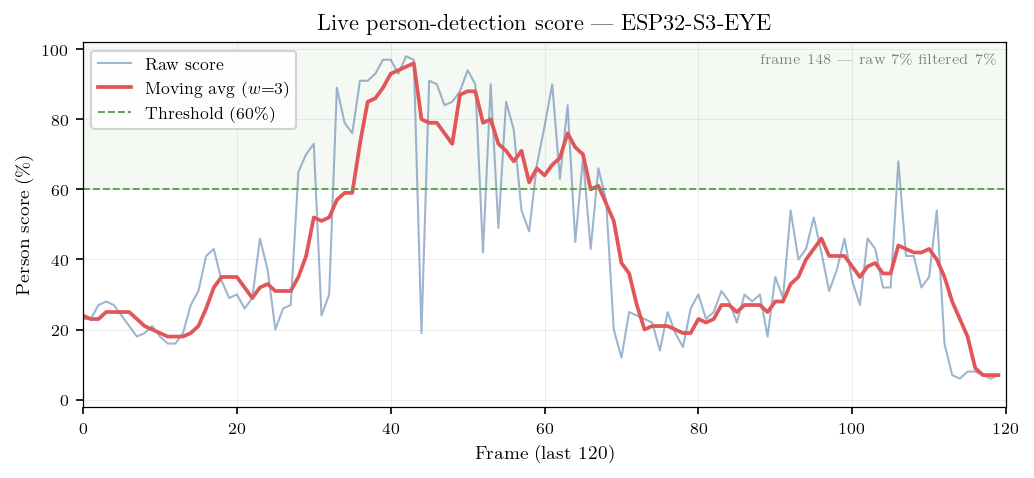
\includegraphics[width=\columnwidth]{Figure_1.png}
  \caption{Raw per-frame person score (blue) and its 3-frame
           moving average (red) recorded on the ESP32-S3-EYE during
           a live session. The green dashed line marks the alarm
           threshold $\theta=0.70$. The filter attenuates transient
           spikes visible in the raw signal while preserving the
           sustained detection event around frames 50--80.}
  \label{fig:livescore}
\end{figure}

\subsection{Python Backend and Telegram Notification}

A Python script subscribes to the MQTT topic via \texttt{paho-mqtt}.
On each alarm message it validates the JSON payload, plays a local
audio alert, and dispatches a real-time notification via the Telegram
Bot API. Telegram was selected as the notification channel for its
widespread adoption, free and well-documented REST API, and
sub-second delivery latency over mobile data. The backend calls the
\texttt{sendMessage} endpoint of the Bot API over HTTPS, delivering a
formatted message containing the event ID, detection confidence, and
local timestamp to a configured chat. All credentials, including the
broker address, bot token, and target chat ID, are passed via
environment variables to avoid hardcoding sensitive information in the
source code.

% ─────────────────────────────────────────────────────────────────────────────
\section{Experimental Results}
\label{sec:results}

\subsection{Hardware Inference Latency}

Inference timing was collected on the deployed device (Xtensa~LX7 @
240\,MHz, \texttt{CONFIG\_NN\_OPTIMIZED} enabled) over $n\!=\!1{,}479$
consecutive frames. Results are shown in Table~\ref{tab:hw_latency} and
Fig.~\ref{fig:latency_box}.

\begin{table}[h]
\centering
\caption{Inference latency on ESP32-S3-EYE ($n\!=\!1{,}479$ frames).}
\label{tab:hw_latency}
\begin{tabular}{@{}lrrrr@{}}
\toprule
\textbf{Layer group} & \textbf{Mean} & \textbf{Std} & \textbf{Min} & \textbf{P99} \\
\midrule
Conv2D (3x3 and all 1x1)     & 323.4\,ms & 0.91\,ms & 321\,ms & 325\,ms \\
DepthwiseConv2D  &  26.6\,ms & 0.54\,ms &  26\,ms &  28\,ms \\
Other layers     & \multicolumn{4}{c}{$<$1\,ms (negligible)} \\
\midrule
\textbf{Total Invoke()} & \textbf{351.3\,ms} & \textbf{0.98\,ms}
  & \textbf{349\,ms} & \textbf{353\,ms} \\
\bottomrule
\end{tabular}
\end{table}

Conv2D operations (the single opening layer plus the 13 pointwise
$1{\times}1$ convolutions inside the depthwise separable blocks)
account for ${\approx}92\,\%$ of total invoke time, while
DepthwiseConv2D contributes the remaining ${\approx}8\,\%$.
A second session ($n\!=\!1{,}560$ frames, \texttt{arch\_log.csv})
collected per-block latency using the firmware architecture profiler;
results are reported in Table~\ref{tab:arch_latency} and
Fig.~\ref{fig:latency_box}.
The opening $3{\times}3$ Conv contributes only 5.1\,ms (1.5\,\%);
the 13 depthwise separable blocks collectively dominate at
${\approx}341\,\text{ms}$ (${\approx}97\,\%$).
Early blocks operating on larger spatial feature maps are markedly
slower: DS\,1 ($80{\times}80$ activations) takes 41.5\,ms and
DS\,3 ($48{\times}48$) takes 39.4\,ms, compared to ${\approx}26.6$\,ms
for mid-network blocks (DS\,7--DS\,11, all at $24{\times}24$) and
13.5\,ms for DS\,12 ($12{\times}12$).
The total latency of 351\,ms corresponds to ${\approx}2.85$\,FPS.

\begin{table}[h]
\centering
\caption{Per-block mean latency on ESP32-S3-EYE ($n\!=\!1{,}560$ frames,
         \texttt{arch\_log.csv}).}
\label{tab:arch_latency}
\resizebox{\columnwidth}{!}{%
\begin{tabular}{@{}lrrrr@{}}
\toprule
\textbf{Block} & \textbf{Mean (ms)} & \textbf{Std (ms)}
  & \textbf{Min (ms)} & \textbf{\% total} \\
\midrule
Conv $3{\times}3$ (opening) &  5.1 & 0.20 & 5.0 &  1.5 \\
DS\,1  & 41.5 & 0.37 & 40.8 & 11.8 \\
DS\,2  & 27.6 & 0.57 & 26.7 &  7.8 \\
DS\,3  & 39.4 & 0.73 & 38.2 & 11.2 \\
DS\,4  & 19.5 & 0.50 & 18.8 &  5.5 \\
DS\,5  & 30.7 & 0.38 & 30.1 &  8.7 \\
DS\,6  & 15.4 & 0.28 & 15.0 &  4.4 \\
DS\,7  & 26.7 & 0.34 & 26.3 &  7.6 \\
DS\,8  & 26.6 & 0.30 & 26.3 &  7.6 \\
DS\,9  & 26.6 & 0.27 & 26.3 &  7.5 \\
DS\,10 & 26.6 & 0.29 & 26.3 &  7.5 \\
DS\,11 & 26.6 & 0.29 & 26.3 &  7.5 \\
DS\,12 & 13.5 & 0.21 & 13.4 &  3.8 \\
DS\,13 & 26.3 & 0.30 & 26.1 &  7.5 \\
GAP + other & 0.3 & 0.03 & 0.3 &  0.1 \\
\midrule
\textbf{Total} & \textbf{352.6} & \textbf{1.03} & \textbf{349.6}
  & \textbf{100} \\
\bottomrule
\end{tabular}%
}
\end{table}

\begin{figure}[h]
  \centering
  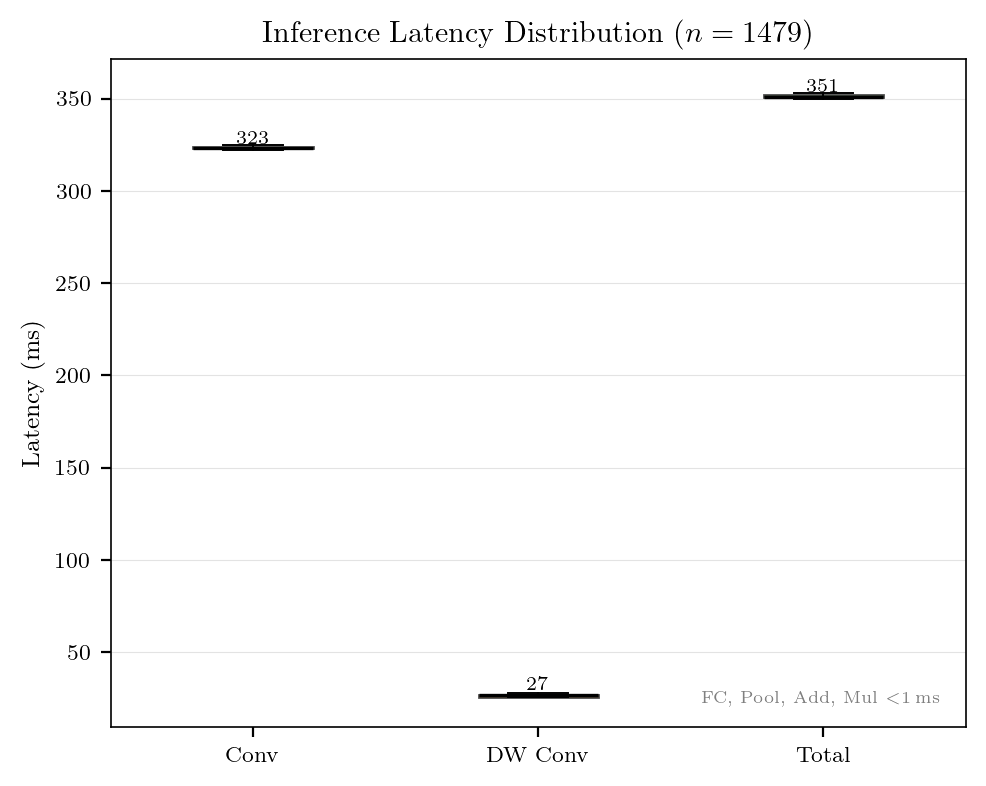
\includegraphics[width=\columnwidth]{stats_boxplot.png}
  \caption{Inference latency distribution ($n\!=\!1{,}479$ frames).
           Conv and DW Conv account for ${\approx}92\,\%$ and
           ${\approx}8\,\%$ of total invoke time, respectively.
           FC, Pool, Add, and Mul are below 1\,ms.}
  \label{fig:latency_box}
\end{figure}

\begin{figure}[h]
  \centering
  \begin{minipage}[t]{0.435\columnwidth}
    \centering
    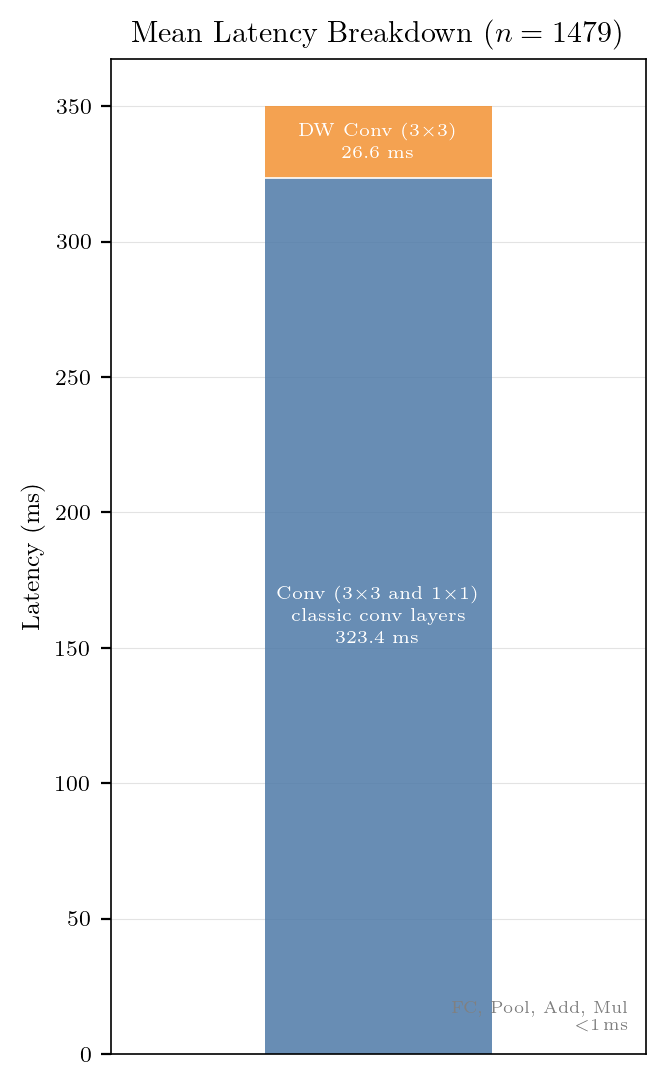
\includegraphics[width=\linewidth]{stats_breakdown.png}
    \caption{Mean latency breakdown by layer type. Conv2D (opening
             $3{\times}3$ plus thirteen $1{\times}1$ PW blocks)
             dominates at ${\approx}323$\,ms; DW Conv contributes
             ${\approx}27$\,ms.}
    \label{fig:latency_breakdown}
  \end{minipage}
  \hfill
  \begin{minipage}[t]{0.505\columnwidth}
    \centering
    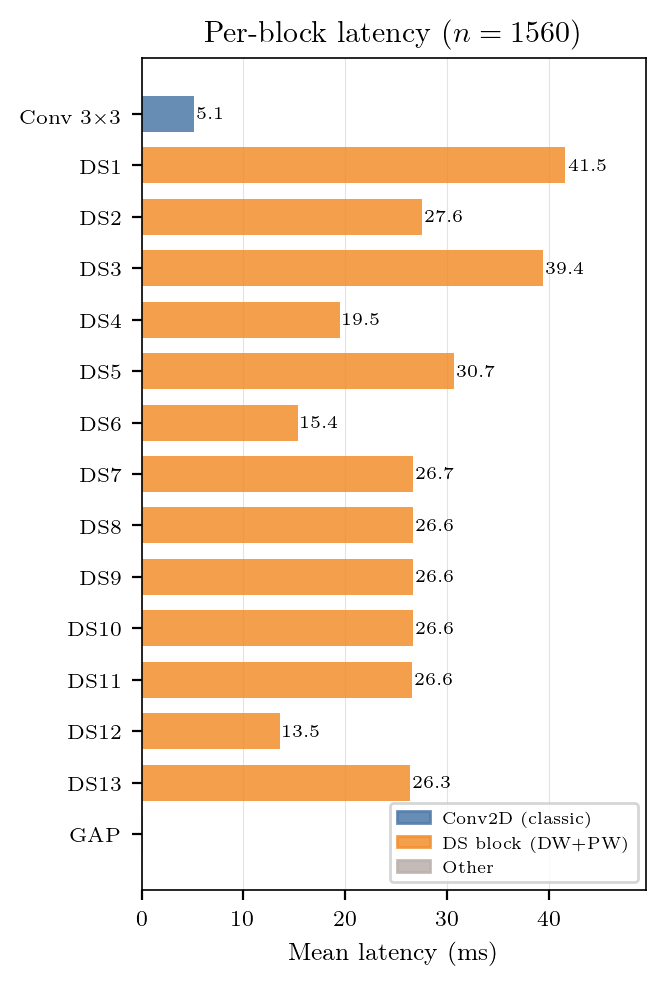
\includegraphics[width=\linewidth]{stats_plot_layer.png}
    \caption{Per-block mean latency. Early DS blocks (DS\,1--3) operating
             on larger feature maps are up to $3{\times}$ slower than
             later ones. Conv $3{\times}3$ contributes only 5.1\,ms
             (${\approx}1.5\,\%$).}
    \label{fig:latency_layer}
  \end{minipage}
\end{figure}

\subsection{Model Efficiency Metrics}

Table~\ref{tab:efficiency} summarises the TinyML efficiency metrics for
the deployed model, extracted via \texttt{model\_efficiency.py}
(included in the repository). \#Parameters counts all weight and bias
tensors reported by the TFLite interpreter. Model size is taken directly
from the C-array length in \texttt{person\_detect\_model\_data.cc}.
Estimated MACs follow analytically from Eq.~(\ref{eq:dwsep}) applied
to each layer of the MobileNetV1 ($\alpha{=}0.25$) graph.

\begin{table}[h]
\centering
\caption{TinyML efficiency metrics for the deployed MobileNetV1 model.}
\label{tab:efficiency}
\begin{tabular}{@{}lr@{}}
\toprule
\textbf{Metric} & \textbf{Value} \\
\midrule
Input resolution        & $96{\times}96$, grayscale, int8 \\
\#Parameters            & 213{,}272 \\
Model size (int8, flash)& 293.5\,KB \\
Float32 equivalent      & 1{,}174\,KB ($4{\times}$ larger) \\
Estimated MACs          & $\approx$7.2\,MMAC \\
Estimated FLOPs         & $\approx$14.3\,MFlop \\
Tensor arena (PSRAM)    & 100\,KB \\
Inference latency (mean)& 351.3\,ms \\
Throughput              & 2.85\,FPS \\
\bottomrule
\end{tabular}
\end{table}

As noted in \cite{mcunet}, on MCUs the \emph{activation memory}
(tensor arena) is the binding constraint, not parameter storage.
The 100\,KB arena accommodates the peak intermediate feature maps,
the largest of which occur after the first standard convolution
($48{\times}48{\times}8 = 18{,}432$ elements) and decrease as spatial
resolution is halved by strided layers.

\subsection{Detection Quality}

The deployed \texttt{.tflite} model was evaluated on 123{,}287 images
from COCO\,2017 (val\,+\,train), labelled in the Visual Wake Words
(person / no-person) layout \cite{vww}. Preprocessing replicates the
firmware pipeline: BT.601 luma conversion and signed-8-bit quantisation.

\begin{table}[h]
\centering
\caption{Classifier performance on 123{,}287 COCO\,2017 images at
         representative thresholds.}
\label{tab:thresholds}
\resizebox{\columnwidth}{!}{%
\begin{tabular}{@{}ccccccc@{}}
\toprule
$\boldsymbol{\theta}$ & \textbf{Prec.} & \textbf{Rec.} & \textbf{F1} &
  \textbf{Acc.} & \textbf{FAR} & \textbf{Profile} \\
\midrule
0.21 & 64.8\,\% & 90.7\,\% & 0.756 & 68.3\,\% & 58.1\,\% & High recall \\
0.26 & 68.2\,\% & 86.1\,\% & \textbf{0.761} & 70.7\,\% & 47.5\,\% & Max F1 \\
\textbf{0.70} & \textbf{88.9\,\%} & \textbf{49.3\,\%} & \textbf{0.634}
  & \textbf{69.2\,\%} & \textbf{7.30\,\%} & \textbf{Firmware default} \\
0.92 & 98.3\,\% & 20.3\,\% & 0.337 & 56.6\,\% & 0.41\,\% & High precision \\
\bottomrule
\end{tabular}%
}
\end{table}

Overall, ROC-AUC\,=\,0.814 and AP\,=\,0.852 (Figs.~\ref{fig:roc}--\ref{fig:sweep})
confirm good discriminative capacity despite int8 quantisation. The
firmware-default $\theta\!=\!0.70$ was selected by combining
benchmark results with on-site validation in a typical indoor
environment: thresholds below ${\approx}0.65$ produced false alarms
on low-texture scenes (e.g.\ ceiling, blank walls), indicating a
positive bias in featureless inputs.
At $\theta\!=\!0.70$, precision is 88.9\,\% with FAR\,=\,7.3\,\%.
Per-frame recall (49.3\,\%) is partially compensated by the moving-average
filter: on sustained person presence consecutive frames produce correlated
high scores that consistently exceed the threshold, while isolated false
positives are averaged down by surrounding low-score frames, effectively
reducing the live false-alarm rate below the per-frame FAR reported here.

The 10\,s cooldown gate is orthogonal to $\theta$ and prevents MQTT
flooding during sustained presence, also this parameter is tunable.

Fig.~\ref{fig:cm} shows the confusion matrices at four representative thresholds. At the firmware default $\theta{=}0.70$ (bottom-left panel), false negatives (missed detections) far outnumber false positives, meaning the system errs toward silence rather than spurious alarms. It is also worth noting that the benchmark dataset (COCO 2017) spans a wide variety of scenes and scenarios, most of which are not surveillance-typical. Moreover, the images are predominantly 4:3 landscape, so the mandatory square-crop resizing distorts person silhouettes, a consequence of replicating the original TFLite Micro training policy, from which this model is shipped \cite{esptflitemicro}. Benchmark accuracy may therefore differ from real deployments where the camera field of view naturally approximates a square crop around the subject. A re-evaluation on a dataset specific to indoor and outdoor surveillance scenarios would provide a more representative estimate of operational performance.

\begin{figure}[h]
  \centering
  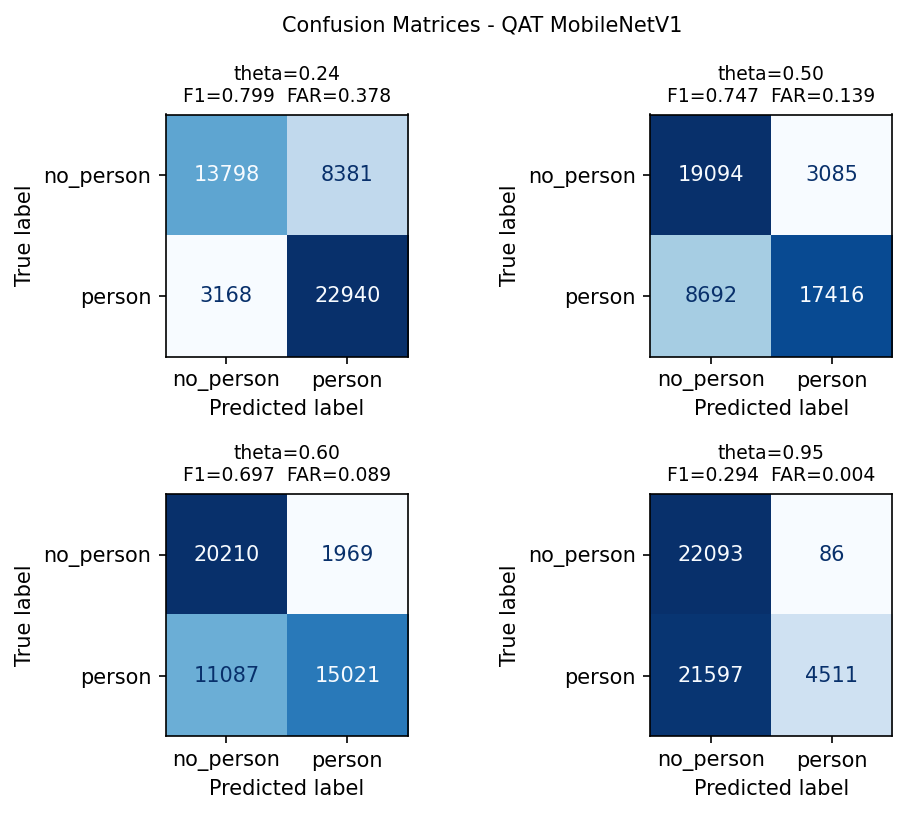
\includegraphics[width=\columnwidth]{confusion_matrix.png}
  \caption{Confusion matrices at $\theta \in \{0.26, 0.50, 0.70, 0.92\}$.
           Bottom-left: firmware default $\theta{=}0.70$.}
  \label{fig:cm}
\end{figure}

\begin{figure}[t]
  \centering
  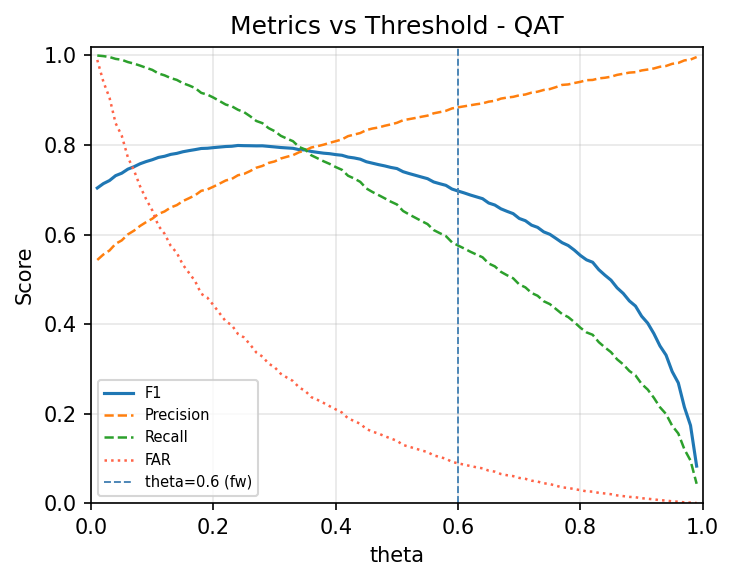
\includegraphics[width=\columnwidth]{threshold_sweep.png}
  \caption{F1, Precision, Recall, and FAR vs.\ threshold $\theta$.
           Vertical marker: firmware default ($\theta\!=\!0.70$).}
  \label{fig:sweep}
\end{figure}

\begin{figure}[t]
  \centering
  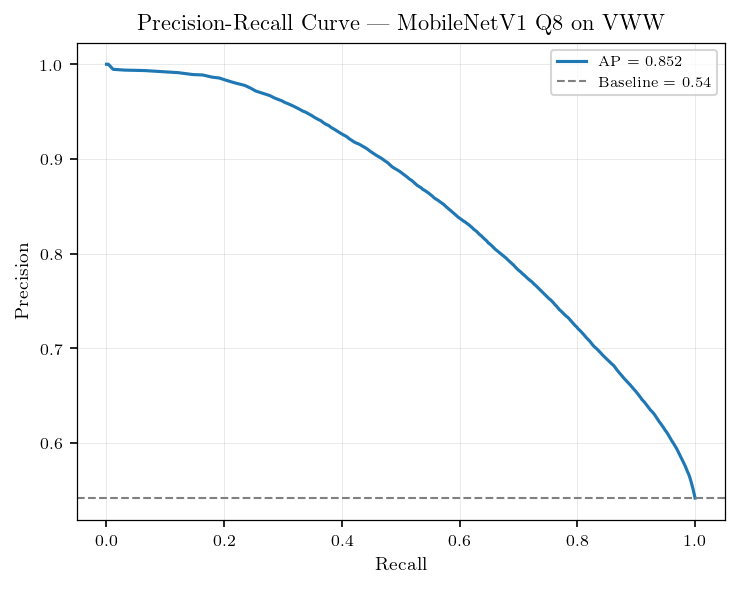
\includegraphics[width=\columnwidth]{pr_curve.png}
  \caption{Precision-Recall curve (AP\,=\,0.852).}
  \label{fig:pr}
\end{figure}

\begin{figure}[t]
  \centering
  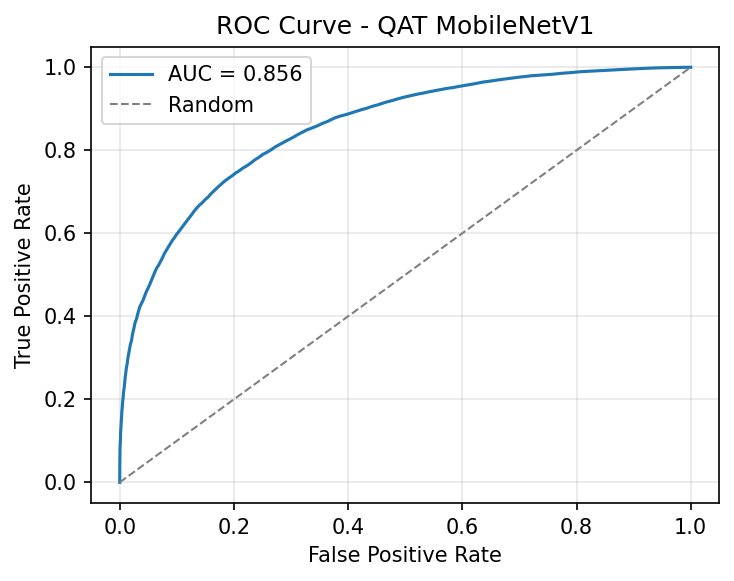
\includegraphics[width=\columnwidth]{roc_curve.png}
  \caption{ROC curve (AUC\,=\,0.814). Dashed diagonal: random classifier.}
  \label{fig:roc}
\end{figure}

% ─────────────────────────────────────────────────────────────────────────────
\section{MobileNetV2 Upgrade Evaluation}
\label{sec:v2}

This section evaluates the impact of replacing the shipped MobileNetV1
($\alpha{=}0.25$, $96{\times}96$ grayscale) with a quantized
MobileNetV2 ($160{\times}160$ RGB, int8) on the same hardware target and
dataset.  The MobileNetV2 architecture introduces inverted residual
blocks with linear bottlenecks~\cite{mobilenetv2}: a $1{\times}1$
\emph{expand} convolution increases the channel count by an expansion
factor $t$, a $3{\times}3$ depthwise convolution operates in the
high-dimensional space, and a $1{\times}1$ \emph{project} convolution
reduces back to a lower-dimensional output without a non-linearity
(the \emph{linear bottleneck}).  Residual shortcuts connect input and
output whenever their shapes match.  The deployed variant uses
$160{\times}160$ RGB int8 input and produces a 2-class output over
$5{\times}5$ spatial positions fed directly to a fully-connected
classifier (no global average pooling), giving $5{\times}5{\times}1280
= 32{,}000$ input units to the final layer.

\subsection{Model Efficiency}

Table~\ref{tab:v2_efficiency} compares the TinyML efficiency metrics
of both models.  MACs for MobileNetV2 were derived analytically by
accumulating $C_\text{out}{\times}K_h{\times}K_w{\times}C_\text{in}%
{\times}H_\text{out}{\times}W_\text{out}$ over every layer of the
17-block backbone plus the closing $1{\times}1$ convolution and
the fully-connected head; spatial dimensions were traced from the
$160{\times}160$ input through the known stride pattern.

\begin{table}[h]
\centering
\caption{TinyML efficiency metrics: MobileNetV1 vs.\ MobileNetV2.
         V2 latency measured on-device ($n\!=\!96$ frames,
         \texttt{latency\_log.csv}).}
\label{tab:v2_efficiency}
\resizebox{\columnwidth}{!}{%
\begin{tabular}{@{}lrr@{}}
\toprule
\textbf{Metric} & \textbf{MobileNetV1} & \textbf{MobileNetV2} \\
\midrule
Input resolution        & $96{\times}96$, gray, int8  & $160{\times}160$, RGB, int8 \\
\#Parameters            & 213{,}272  & 453{,}104 \\
Model size (int8)       & 293.5\,KB  & 664.5\,KB \\
Float32 equivalent      & 1{,}174\,KB & 2{,}658\,KB \\
Estimated MACs          & $\approx$7.2\,MMAC & $\approx$26.7\,MMAC \\
Estimated FLOPs         & $\approx$14.3\,MFlop & $\approx$53.3\,MFlop \\
Tensor arena (PSRAM)    & 100\,KB     & 900\,KB \\
Inference latency (mean)& 351.3\,ms  & 1{,}919.4\,ms \\
Inference latency (std) & 0.98\,ms   & 0.71\,ms \\
Inference latency (min) & 349\,ms    & 1{,}919\,ms \\
Inference latency (P99) & 353\,ms    & 1{,}921\,ms \\
Throughput              & 2.85\,FPS  & 0.52\,FPS \\
\bottomrule
\end{tabular}%
}
\end{table}

The V2 model is $2.3{\times}$ larger on flash, carries $2.1{\times}$ more
parameters, and requires $3.7{\times}$ more multiply-accumulate operations
than V1.  This stems primarily from the larger input resolution
($160{\times}160$ vs.\ $96{\times}96$, a $2.78{\times}$ area increase)
and the three-channel RGB input (vs.\ single-channel grayscale), both of
which multiply the workload of the early convolutional layers.
The tensor arena grows from 100\,KB to 900\,KB, driven by the peak
activation map after the opening convolution
($80{\times}80{\times}16 = 102{,}400$ int8 elements) and the accumulated
intermediate feature maps of the wider bottleneck blocks.

On-device measurement ($n\!=\!96$ frames, Xtensa~LX7 @ 240\,MHz,
\texttt{CONFIG\_NN\_OPTIMIZED} enabled) confirms a mean inference
latency of $1{,}919.4$\,ms ($\sigma\!=\!0.71$\,ms), corresponding to
$\approx0.52$\,FPS --- a $5.46{\times}$ slowdown relative to V1.
The extremely low variance ($<1$\,ms) reflects the fully deterministic
execution of quantized kernels on SRAM-resident activations with no
cache effects.

\subsubsection*{Impact on the moving-average window}

The firmware uses a moving-average filter of window $W$ to suppress
per-frame false positives (Eq.~\ref{eq:mavg}).  At V1's 351\,ms per
frame, $W\!=\!3$ spans $\approx\!1$\,s and adds negligible alarm
latency.  At V2's 1{,}919\,ms per frame, the same window $W\!=\!3$
spans $\approx\!5.8$\,s, and the firmware default $W\!=\!5$ spans
$\approx\!9.6$\,s worst-case before a sustained detection triggers an
alarm.  For a security application this delay is unacceptable.
Setting $W\!=\!1$ (i.e.\ disabling temporal smoothing entirely)
reduces alarm latency to a single inference cycle ($\approx\!1.9$\,s)
while accepting a marginally higher instantaneous false-positive rate;
at the firmware threshold $\theta\!=\!0.70$ the per-frame FAR of
$50.8\,\%$ makes this trade-off less favourable than for V1, so a
combined approach --- $W\!=\!1$ with a raised threshold
$\theta\!\geq\!0.90$ --- is recommended for V2 deployments until
a VWW-fine-tuned checkpoint is available.

\subsection{Detection Quality}

The int8 model was evaluated on the same 123{,}287 COCO\,2017 images used
for V1, with preprocessing matched to the V2 firmware pipeline:
nearest-neighbour resize to $160{\times}160$ and subtraction of 128 to
convert uint8 RGB to signed 8-bit.

Table~\ref{tab:v2_thresholds} reports classifier performance at four
representative thresholds alongside the corresponding V1 figures for direct
comparison.  Overall, MobileNetV2 achieves ROC-AUC\,=\,0.705 and
AP\,=\,0.699 (Figs.~\ref{fig:v2_roc}--\ref{fig:v2_sweep}), compared to
0.814 and 0.852 for V1.

\begin{table}[h]
\centering
\caption{MobileNetV2 classifier performance on 123{,}287 COCO\,2017 images
         at representative thresholds.  V1 figures from
         Table~\ref{tab:thresholds} are shown in parentheses for comparison.}
\label{tab:v2_thresholds}
\resizebox{\columnwidth}{!}{%
\begin{tabular}{@{}cccccc@{}}
\toprule
$\boldsymbol{\theta}$ & \textbf{Prec.} & \textbf{Rec.} & \textbf{F1} &
  \textbf{FAR} & \textbf{Profile} \\
\midrule
0.07 & 59.9\,\% & 90.1\,\% & 0.720 & 71.3\,\% & High recall \\
0.23 & 61.8\,\% & 86.3\,\% & \textbf{0.721} & 63.0\,\% & Max F1 \\
\textbf{0.70}
  & \textbf{65.0\,\%} \,(88.9\,\%)
  & \textbf{79.8\,\%} \,(49.3\,\%)
  & \textbf{0.716} \,(0.634)
  & \textbf{50.8\,\%} \,(7.3\,\%)
  & \textbf{Firmware default} \\
0.92 & 67.8\,\% & 74.0\,\% & 0.708 & 41.6\,\% & High precision \\
\bottomrule
\end{tabular}%
}
\end{table}

At the firmware-default $\theta{=}0.70$, V2 delivers substantially higher
recall ($79.8\,\%$ vs.\ $49.3\,\%$) but at the cost of a much higher
false-alarm rate ($50.8\,\%$ vs.\ $7.3\,\%$) and lower precision
($65.0\,\%$ vs.\ $88.9\,\%$).  The lower discriminative capacity is
reflected in a $\approx{13}$-point drop in ROC-AUC (0.705 vs.\ 0.814),
suggesting that the deployed MobileNetV2 checkpoint is not fine-tuned on
the Visual Wake Words task: it was trained as a general RGB classifier
and applied here without VWW-specific fine-tuning, whereas the V1 model
was shipped specifically for VWW on the ESP32 platform~\cite{esptflitemicro}.

Notably, the F1 score varies only in the range $[0.708, 0.721]$ across all
thresholds, indicating a nearly flat precision-recall trade-off.  The
threshold $\theta{=}0.70$ would need to be substantially raised (above $0.90$)
to approach V1-level precision, but at the cost of recall dropping below
$75\,\%$.  Alternatively, fine-tuning V2 on the VWW dataset prior to
deployment is the recommended path to recover the V1 precision advantage
while retaining the higher-resolution RGB input capability.

\begin{figure}[h]
  \centering
  
\includegraphics[width=\columnwidth]{mobilenetv2_coco_all/confusion_matrix.png}
  \caption{MobileNetV2 confusion matrices at
           $\theta \in \{0.25,\,0.50,\,0.70,\,0.90\}$.}
  \label{fig:v2_cm}
\end{figure}

\begin{figure}[h]
  \centering
  
\includegraphics[width=\columnwidth]{mobilenetv2_coco_all/threshold_sweep.png}
  \caption{MobileNetV2: F1, Precision, Recall, and FAR vs.\ $\theta$.
           Note the near-flat F1 across the full threshold range.}
  \label{fig:v2_sweep}
\end{figure}

\begin{figure}[h]
  \centering
  
\includegraphics[width=\columnwidth]{mobilenetv2_coco_all/pr_curve.png}
  \caption{MobileNetV2 Precision-Recall curve (AP\,=\,0.699).}
  \label{fig:v2_pr}
\end{figure}

\begin{figure}[h]
  \centering
  
\includegraphics[width=\columnwidth]{mobilenetv2_coco_all/roc_curve.png}
  \caption{MobileNetV2 ROC curve (AUC\,=\,0.705).}
  \label{fig:v2_roc}
\end{figure}

% ─────────────────────────────────────────────────────────────────────────────
\newpage
\section{Conclusion}
\label{sec:conclusion}

This paper presented a complete Smart Visual Alarm System running fully on the
ESP32-S3-EYE: on-device TFLite Micro inference, moving-average alarm
logic, MQTT\,QoS\,1 event publication, and Python/Telegram notification.
Raw video is never transmitted: only compact JSON descriptors leave the
device. Evaluation on 123{,}287 COCO\,2017 images yields
ROC-AUC\,=\,0.814 and AP\,=\,0.852. The firmware threshold
$\theta\!=\!0.70$ provides 88.9\,\% precision at 7.3\,\% FAR, and the
three-frame moving-average filter further reduces the effective false-alarm
rate on live video.

Future work includes: upgrading to MCUNet \cite{mcunet} for improved
recall at lower memory cost, re-benchmarking on a surveillance-specific
dataset (covering typical indoor and outdoor camera viewpoints) to obtain
accuracy estimates more representative of operational deployments,
NTP clock synchronisation, TLS on MQTT
and encrypted NVS for credentials, and deep-sleep duty cycling for
battery operation.

% ─────────────────────────────────────────────────────────────────────────────
\begin{thebibliography}{00}

\bibitem{esp32s3eye}
Espressif Systems, ``ESP32-S3-EYE Getting Started Guide,'' 2022.
[Online]. Available: \url{https://github.com/espressif/esp-who}

\bibitem{tflitemicro}
R.~David \textit{et al.}, ``TensorFlow Lite Micro: Embedded Machine
Learning on TinyML Systems,'' in \textit{Proc.\ MLSys}, 2021.

\bibitem{esptflitemicro}
Espressif Systems, ``esp-tflite-micro,'' GitHub, 2023.
[Online]. Available: \url{https://github.com/espressif/esp-tflite-micro}

\bibitem{vww}
A.~Chowdhery \textit{et al.}, ``Visual Wake Words Dataset,''
\textit{arXiv:1906.05721}, 2019.

\bibitem{mobilenet}
A.~Howard \textit{et al.}, ``MobileNets: Efficient Convolutional Neural
Networks for Mobile Vision Applications,'' \textit{arXiv:1704.04861}, 2017.

\bibitem{mcunet}
J.~Lin \textit{et al.}, ``MCUNet: Tiny Deep Learning on IoT Devices,''
in \textit{NeurIPS}, 2020.

\bibitem{mobilenetv2}
M.~Sandler \textit{et al.}, ``MobileNetV2: Inverted Residuals and Linear
Bottlenecks,'' in \textit{Proc.\ CVPR}, 2018.

\bibitem{ftc2023ring}
Federal Trade Commission, ``FTC Says Ring Employees Illegally Surveilled Customers, Failed to Stop Hackers from Taking Control of Users' Cameras,'' Press Release, May 2023. [Online]. Available: \url{https://www.ftc.gov/news-events/news/press-releases/2023/05/ftc-says-ring-employees-illegally-surveilled-customers-failed-stop-hackers-taking-control-users}

\end{thebibliography}

\end{document}